\documentclass{article}[18pt]
\usepackage[utf8]{inputenc}
\usepackage[margin=0.7in]{geometry}
\usepackage{parselines} 
\usepackage{amsmath}
\usepackage{titlesec}
\usepackage{pgfplots}
\usepackage{graphicx}
\usepackage[english]{babel}
\usepackage{fancyhdr}
\usepackage{amssymb}
\pgfplotsset{width=10cm,compat=1.9}
\usepackage{mwe}
\usepackage{float}


\titlespacing\section{0pt}{14pt plus 4pt minus 2pt}{0pt plus 2pt minus 2pt}
\newlength\tindent
\setlength{\tindent}{\parindent}
\setlength{\parindent}{0pt}
\renewcommand{\indent}{\hspace*{\tindent}}

\pagestyle{fancy}
\fancyhf{}
\rhead{Sam Robbins 13SE}
\lhead{A Level Maths - C3}
%\rfoot{Page \thepage}

\newcommand{\R}{\mathbb{R}}
\pgfplotsset{ytick style={draw=none}}
\pgfplotsset{xtick style={draw=none}}
\renewcommand{\arraystretch}{3}

\begin{document}
\begin{center}
\underline{\huge C3}
\end{center}
\begin{obeylines}

\section{Algebraic fractions}
Any polynomial $F(x)$ can be put in the form:
$F(x)=Q(x)\times$divisor+remainder
Where Q(x) is the quotient
\section{Functions}
\subsection{Range and domain}
The input to a function is the \textbf{Domain}\\
The output from a function is the \textbf{Range}
\subsection{Function mapping}
One-to-one function: One element in the domain maps to one element in the range
Many-to-one function: To elements of the domain maps to one element in the range
Not a function: One input maps to two outputs
\subsection{Mappings to functions by changing the domain}
Consider $y=\sqrt{x}$
If the domain is all the real numbers $x \in \Re$ then it is not a function as values less than 0 don't get mapped anywhere.
The domain must be restricted to $x\geq 0$
\subsection{Combining functions}
$fg(x)$ means apply g to x, then apply f
$f^2(x)$ means $ff(x)$
\subsection{Inverse functions}
The inverse of $f(x)$ is written as $f^{-1}x$
The domain of $f(x)$ is the range of $f^{-1}x$
The range of $f(x)$ is the domain of $f^{-1}x$

Example, find the inverse function of $y=2x^2-7$:
$y+7=2x^2$\\
$\dfrac{y+7}{2}=x^2$\\
$x=\sqrt{\dfrac{y+7}{2}}$\\
$f^{-1}x=\sqrt{\dfrac{x+7}{2}}$\\

When finding the graph of an inverse function, reflect $f(x)$ in the line y=x.

\section{The exponential and log functions}
\subsection{Exponential functions}
Exponential functions are in the form $y=a^x$, graphs of these functions all pass through (0,1) as $a^0=1$ for any value of a.
\subsection{Functions including e}
The function $y=e^x$ is the function where the gradient is identical to the function.
$y=e^x \dfrac{dy}{dx}=e^x$
\newpage
Below is the graph of $y=e^x$
\begin{tikzpicture}[scale=0.5]
\begin{axis}[ymin=0]
\addplot[color=black,domain=-2:2]{exp(x)};
\draw[ultra thin] (axis cs:0,\pgfkeysvalueof{/pgfplots/ymin}) -- (axis cs:0,\pgfkeysvalueof{/pgfplots/ymax});
\draw[ultra thin] (axis cs:\pgfkeysvalueof{/pgfplots/xmin},0) -- (axis cs:\pgfkeysvalueof{/pgfplots/xmax},0);

\end{axis}
\end{tikzpicture}
$y=e^{-x}$
\begin{tikzpicture}[scale=0.5]
\begin{axis}[ymin=0]
\addplot[color=black, domain=-2:2]{1/exp(x)};
\draw[ultra thin] (axis cs:0,\pgfkeysvalueof{/pgfplots/ymin}) -- (axis cs:0,\pgfkeysvalueof{/pgfplots/ymax});
\draw[ultra thin] (axis cs:\pgfkeysvalueof{/pgfplots/xmin},0) -- (axis cs:\pgfkeysvalueof{/pgfplots/xmax},0);

\end{axis}
\end{tikzpicture}

$y=e^{2x}$ (black) $y=e^x$ (red)
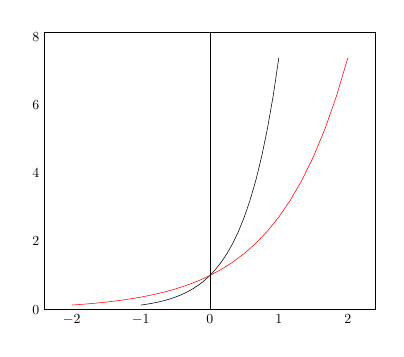
\begin{tikzpicture}[scale=0.5]
\begin{axis}[ymin=0]
\addplot[color=black,domain=-1:1, ]{e^(2*x)};
\addplot[color=red,domain=-2:2, ]{exp(x)};
\draw[ultra thin] (axis cs:0,\pgfkeysvalueof{/pgfplots/ymin}) -- (axis cs:0,\pgfkeysvalueof{/pgfplots/ymax});
\draw[ultra thin] (axis cs:\pgfkeysvalueof{/pgfplots/xmin},0) -- (axis cs:\pgfkeysvalueof{/pgfplots/xmax},0);

\end{axis}
\end{tikzpicture}

$y=10e^{-x}$ (black) $y=e^{-x}$ (red)
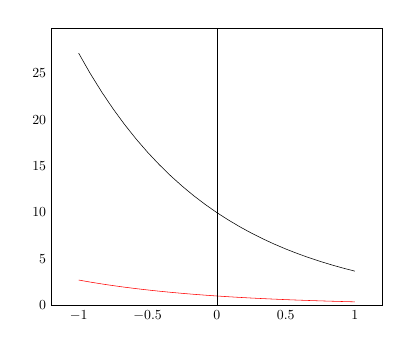
\begin{tikzpicture}[scale=0.5]
\begin{axis}[ymin=0]
\addplot[color=black,domain=-1:1]{(10*(e^(-x)))};
\addplot[color=red,domain=-1:1]{1/e^(x)};
\draw[ultra thin] (axis cs:0,\pgfkeysvalueof{/pgfplots/ymin}) -- (axis cs:0,\pgfkeysvalueof{/pgfplots/ymax});
\draw[ultra thin] (axis cs:\pgfkeysvalueof{/pgfplots/xmin},0) -- (axis cs:\pgfkeysvalueof{/pgfplots/xmax},0);

\end{axis}
\end{tikzpicture}

\subsection{Formulas for exponential growth or decay}
Example:
$P=16000e^{-\dfrac{t}{10}}$
Where P is the Price in £s and t is the years from new
\textit{What was the price when new?}
Substitute t=0
$ $
$P=16000e^{-\dfrac{0}{10}}$
$ $
$P=16000 \times 1$
\newpage
\textit{What is the value at 5 years old}
Substitute t=5
$ $
$P=16000e^{-\frac{5}{10}}$
$P=\mathsterling 9704.49$
\textit{What does the model say about the eventual value of the car}
As $t \rightarrow \infty$, $e^{-\frac{t}{10}} \rightarrow \infty$
Therefore $P \rightarrow 16000 \times 0 = 0$
The eventual value is zero.

\subsection{The inverse of the exponential function}
The inverse of $e^x$ is $\log_ex$ (also written as $\ln x$)
Examples:
If $e^x=3$ then $x=\ln3$
If $\ln x=4$ then $x=e^4$
$ $
$y=e^{x}$ (Red) $y=\ln x$ (Black)
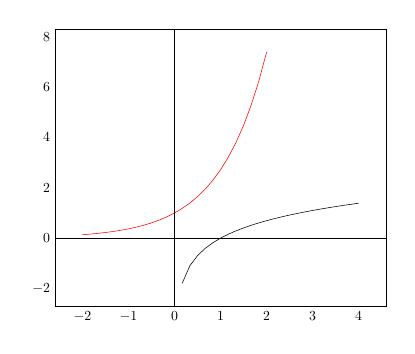
\begin{tikzpicture}[scale=0.5]
\begin{axis}
\addplot[color=black,domain=0:4, ]{ln(x)};
\addplot[color=red,domain=-2:2, ]{exp(x)};
\draw[ultra thin] (axis cs:0,\pgfkeysvalueof{/pgfplots/ymin}) -- (axis cs:0,\pgfkeysvalueof{/pgfplots/ymax});
\draw[ultra thin] (axis cs:\pgfkeysvalueof{/pgfplots/xmin},0) -- (axis cs:\pgfkeysvalueof{/pgfplots/xmax},0);

\end{axis}
\end{tikzpicture}

The function $f(x)=\ln x$ has domain \{$x \in \mathbb{R}$, $x>0$\} and range \{$f(x) \in \mathbb{R}$\}

\section{Numerical methods}
\subsection{Approximations for roots based on graphs}
Approximations for roots can be found graphically by plotting the function and finding where the line crosses the x axis. This value is one of the roots of the function.

If trying to find a range in which a root can be found, substitute the values at the extreme of the range, and if there is a change in sign between the two results, there will be a root in the range.

The exception to this rule is $f(x)=\dfrac{1}{x}$ and transformations of this as there is a discontinuity at x=0. The function changes sign in the interval that includes x=0, but there is not a root.

\subsection{Iteration for finding approximations of roots}
To solve an equation of the form $f(x)=0$ by an iterative method, rearrange $f(x)=0$ into a for $x=g(x)$ and use the iterative formula $x_{n+1}=g(x_n)$.
$ $


Example, find a root of the equation $x^2-4x+1=0$
Re-write as $x=4-\dfrac{1}{x}$

Create the formula $x_{n+1}=4-\dfrac{1}{x_n}$
You get given a rough approximation, $x_0=3$
Substitute
$x_1=4-\dfrac{1}{x_0}$
$x_1=4-\dfrac{1}{3}$
$x_1=\dfrac{11}{3}$
$ $
$x_2=4-\dfrac{1}{\frac{11}{3}}$
$x_2=\dfrac{41}{11}$
Continuing this increases the accuracy of the result.
This may not work and will not converge to a root.
\section{Transforming graphs of functions}
\subsection{$\mathbf{y=|f(x)|}$ Graphs}
The modulus of a number is written as $|a|$, this is the positive numerical value.
When $f(x) \geq 0, |f(x)|=f(x)$
When $f(x)<0, |f(x)|=-f(x)$
$ $


\end{obeylines}


\begin{figure}[H]
    \centering
    \begin{minipage}{0.45\textwidth}
        \centering
        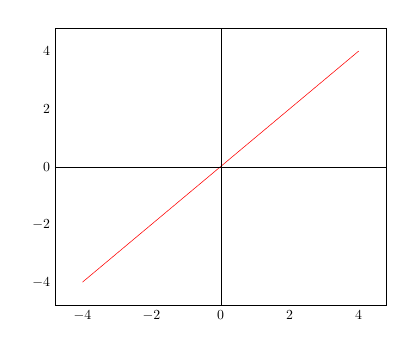
\begin{tikzpicture}[scale=0.5]
\begin{axis}[]
\addplot[color=red,domain=-4:4, ]{x};
\draw[ultra thin] (axis cs:0,\pgfkeysvalueof{/pgfplots/ymin}) -- (axis cs:0,\pgfkeysvalueof{/pgfplots/ymax});
\draw[ultra thin] (axis cs:\pgfkeysvalueof{/pgfplots/xmin},0) -- (axis cs:\pgfkeysvalueof{/pgfplots/xmax},0);
\end{axis}
\end{tikzpicture}
        \caption{$y=x$}
    \end{minipage}\hfill
    \begin{minipage}{0.45\textwidth}
        \centering
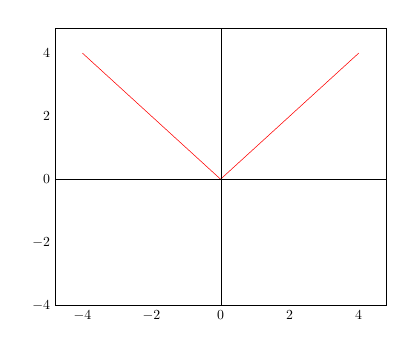
\begin{tikzpicture}[scale=0.5]
\begin{axis}[ymin=-4]
\addplot[color=red,domain=-4:4, ]{abs(x)};
\draw[ultra thin] (axis cs:0,\pgfkeysvalueof{/pgfplots/ymin}) -- (axis cs:0,\pgfkeysvalueof{/pgfplots/ymax});
\draw[ultra thin] (axis cs:\pgfkeysvalueof{/pgfplots/xmin},0) -- (axis cs:\pgfkeysvalueof{/pgfplots/xmax},0);
\end{axis}
\end{tikzpicture}      
        \caption{$y=|x|$}
    \end{minipage}
\end{figure}


\begin{figure}[H]
    \centering
    \begin{minipage}{0.45\textwidth}
        \centering
\begin{tikzpicture}[scale=0.5]
\begin{axis}[ymin=-10,ymax=10]
\addplot[color=red,domain=-2:3, ]{3*x-2};
\draw[ultra thin] (axis cs:0,\pgfkeysvalueof{/pgfplots/ymin}) -- (axis cs:0,\pgfkeysvalueof{/pgfplots/ymax});
\draw[ultra thin] (axis cs:\pgfkeysvalueof{/pgfplots/xmin},0) -- (axis cs:\pgfkeysvalueof{/pgfplots/xmax},0);
\end{axis}
\end{tikzpicture}
        \caption{$y=3x-2$}
    \end{minipage}\hfill
    \begin{minipage}{0.45\textwidth}
        \centering
\begin{tikzpicture}[scale=0.5]
\begin{axis}[ymin=-10,ymax=10]
\addplot[color=red,domain=-2:3,samples=300 ]{abs(3*x-2)};
\draw[ultra thin] (axis cs:0,\pgfkeysvalueof{/pgfplots/ymin}) -- (axis cs:0,\pgfkeysvalueof{/pgfplots/ymax});
\draw[ultra thin] (axis cs:\pgfkeysvalueof{/pgfplots/xmin},0) -- (axis cs:\pgfkeysvalueof{/pgfplots/xmax},0);
\end{axis}
\end{tikzpicture}
        \caption{$y=|3x-2|$}
    \end{minipage}
\end{figure}








\begin{figure}[H]
    \centering
    \begin{minipage}{0.45\textwidth}
        \centering
        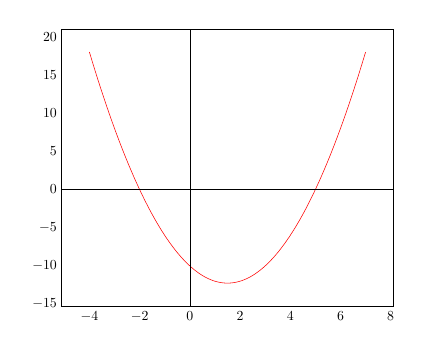
\begin{tikzpicture}[scale=0.5]
\begin{axis}
\addplot[color=red,domain=-4:7,samples=500 ]{x^2-3*x-10};
\draw[ultra thin] (axis cs:0,\pgfkeysvalueof{/pgfplots/ymin}) -- (axis cs:0,\pgfkeysvalueof{/pgfplots/ymax});
\draw[ultra thin] (axis cs:\pgfkeysvalueof{/pgfplots/xmin},0) -- (axis cs:\pgfkeysvalueof{/pgfplots/xmax},0);
\end{axis}
\end{tikzpicture}
        \caption{$y=x^2-3x-10$}
    \end{minipage}\hfill
    \begin{minipage}{0.45\textwidth}
        \centering
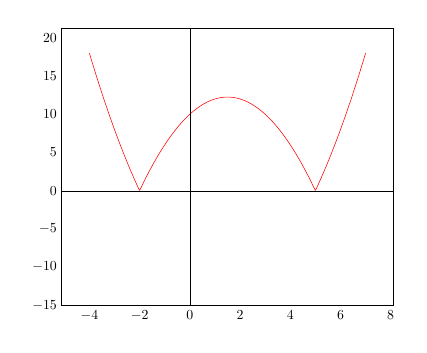
\begin{tikzpicture}[scale=0.5]
\begin{axis}[ymin=-15]
\addplot[color=red,domain=-4:7,samples=500 ]{abs(x^2-3*x-10)};
\draw[ultra thin] (axis cs:0,\pgfkeysvalueof{/pgfplots/ymin}) -- (axis cs:0,\pgfkeysvalueof{/pgfplots/ymax});
\draw[ultra thin] (axis cs:\pgfkeysvalueof{/pgfplots/xmin},0) -- (axis cs:\pgfkeysvalueof{/pgfplots/xmax},0);
\end{axis}
\end{tikzpicture}        
        \caption{$y=|x^2-3x-10|$}
    \end{minipage}
\end{figure}




\begin{figure}[H]
    \centering
    \begin{minipage}{0.45\textwidth}
        \centering
        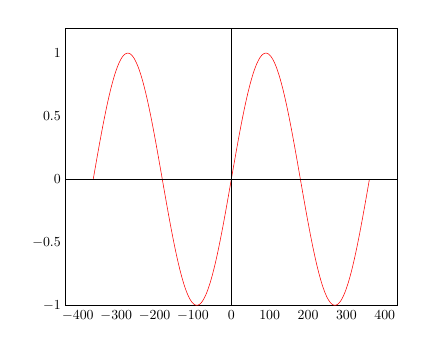
\begin{tikzpicture}[scale=0.5]
\begin{axis}[ymin=-1]
\addplot[color=red,domain=-360:360,samples=500 ]{sin(x)};
\draw[ultra thin] (axis cs:0,\pgfkeysvalueof{/pgfplots/ymin}) -- (axis cs:0,\pgfkeysvalueof{/pgfplots/ymax});
\draw[ultra thin] (axis cs:\pgfkeysvalueof{/pgfplots/xmin},0) -- (axis cs:\pgfkeysvalueof{/pgfplots/xmax},0);
\end{axis}
\end{tikzpicture}
        \caption{$y=sin(x)$}
    \end{minipage}\hfill
    \begin{minipage}{0.45\textwidth}
        \centering
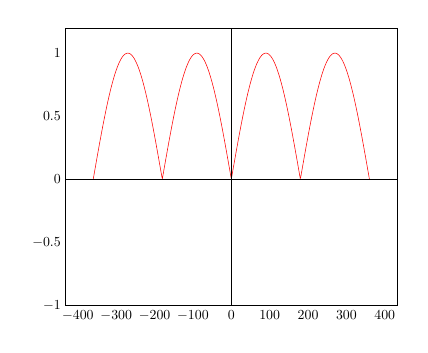
\begin{tikzpicture}[scale=0.5]
\begin{axis}[ymin=-1]
\addplot[color=red,domain=-360:360,samples=500 ]{abs(sin(x))};
\draw[ultra thin] (axis cs:0,\pgfkeysvalueof{/pgfplots/ymin}) -- (axis cs:0,\pgfkeysvalueof{/pgfplots/ymax});
\draw[ultra thin] (axis cs:\pgfkeysvalueof{/pgfplots/xmin},0) -- (axis cs:\pgfkeysvalueof{/pgfplots/xmax},0);
\end{axis}
\end{tikzpicture}        
        \caption{$y=|sin(x)|$}
    \end{minipage}
\end{figure}
        
\subsection{$\mathbf{y=f(|x|)}$ Graphs}
To plot the graph of $y=|x|-2$, first sketch the graph of $y=x-2$ for $x \geq  0$:
\\
        \begin{tikzpicture}[scale=0.5]
\begin{axis}[ymin=-4, xmin=-4, ymax=4, xmax=4]
\addplot[color=red,domain=0:5,samples=100 ]{x-2};
\draw[ultra thin] (axis cs:0,\pgfkeysvalueof{/pgfplots/ymin}) -- (axis cs:0,\pgfkeysvalueof{/pgfplots/ymax});
\draw[ultra thin] (axis cs:\pgfkeysvalueof{/pgfplots/xmin},0) -- (axis cs:\pgfkeysvalueof{/pgfplots/xmax},0);
\end{axis}
\end{tikzpicture}
\\
Then reflect that graph in the y axis
\\
        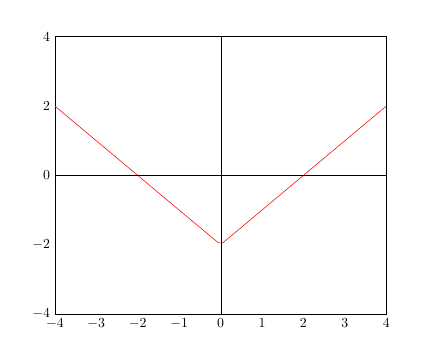
\begin{tikzpicture}[scale=0.5]
\begin{axis}[ymin=-4, xmin=-4, ymax=4, xmax=4]
\addplot[color=red,domain=-5:5,samples=100 ]{abs(x)-2};
\draw[ultra thin] (axis cs:0,\pgfkeysvalueof{/pgfplots/ymin}) -- (axis cs:0,\pgfkeysvalueof{/pgfplots/ymax});
\draw[ultra thin] (axis cs:\pgfkeysvalueof{/pgfplots/xmin},0) -- (axis cs:\pgfkeysvalueof{/pgfplots/xmax},0);
\end{axis}
\end{tikzpicture}
\\
Examples:
\begin{figure}[H]
    \centering
    \begin{minipage}{0.45\textwidth}
        \centering
        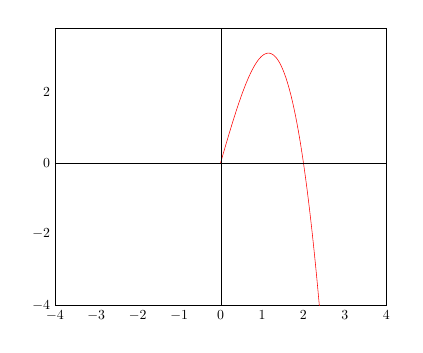
\begin{tikzpicture}[scale=0.5]
\begin{axis}[ymin=-4,xmin=-4,xmax=4]
\addplot[color=red,domain=0:4,samples=500 ]{4*x-x^3};
\draw[ultra thin] (axis cs:0,\pgfkeysvalueof{/pgfplots/ymin}) -- (axis cs:0,\pgfkeysvalueof{/pgfplots/ymax});
\draw[ultra thin] (axis cs:\pgfkeysvalueof{/pgfplots/xmin},0) -- (axis cs:\pgfkeysvalueof{/pgfplots/xmax},0);
\end{axis}
\end{tikzpicture}
        \caption{$y=4x-x^3$}
    \end{minipage}\hfill
    \begin{minipage}{0.45\textwidth}
        \centering
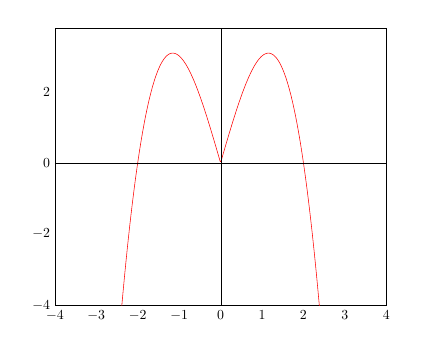
\begin{tikzpicture}[scale=0.5]
\begin{axis}[ymin=-4,xmax=4,xmin=-4]
\addplot[color=red,domain=-4:4,samples=500 ]{4*abs(x)-(abs(x))^3};
\draw[ultra thin] (axis cs:0,\pgfkeysvalueof{/pgfplots/ymin}) -- (axis cs:0,\pgfkeysvalueof{/pgfplots/ymax});
\draw[ultra thin] (axis cs:\pgfkeysvalueof{/pgfplots/xmin},0) -- (axis cs:\pgfkeysvalueof{/pgfplots/xmax},0);
\end{axis}
\end{tikzpicture}        
        \caption{$y=4|x|-{|x|}^3$}
    \end{minipage}
\end{figure}

\subsection{Graph transformations}
\begin{itemize}
\item $f(x+a)$ - Horizontal translation of $\mathbf{-a}$
\item $f(x)+a$ - Vertical translation of $\mathbf{+a}$
\item $f(ax)$ - Horizontal stretch of scale factor $\mathbf{\frac{1}{a}}$
\item $f(-x)$ - Reflection in the \textbf{y axis}
\item $af(x)$ - Vertical stretch of scale factor $\mathbf{a}$
\item $-f(x)$ - Reflection in the \textbf{x axis}
\end{itemize}
\section{Trigonometry}
\begin{itemize}
\item $\sec\theta=\dfrac{1}{\cos\theta}$
\item $\csc\theta=\dfrac{1}{\sin\theta}=cosec\theta$
\item $\cot\theta=\dfrac{1}{\tan\theta}$
\item $\cot\theta=\dfrac{\cos\theta}{\sin\theta}$
\end{itemize}
\subsection{Graphs of the new functions}
$\sec(x)$
\\
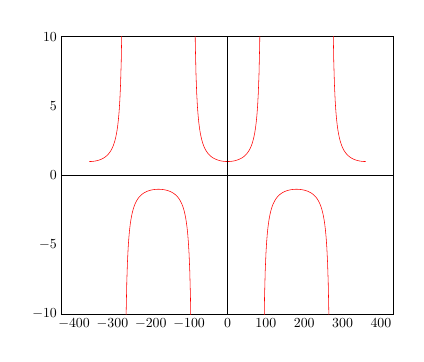
\begin{tikzpicture}[scale=0.5]
\begin{axis}[ymax=10,ymin=-10]
\addplot[color=red,domain=-360:360,samples=400,restrict y to domain=-15:15]
{sec(x)};
\draw[ultra thin] (axis cs:0,\pgfkeysvalueof{/pgfplots/ymin}) -- (axis 
cs:0,\pgfkeysvalueof{/pgfplots/ymax});
\draw[ultra thin] (axis cs:\pgfkeysvalueof{/pgfplots/xmin},0) -- (axis 
cs:\pgfkeysvalueof{/pgfplots/xmax},0);
\end{axis}
\end{tikzpicture}
\\
$\csc(x)$
\\
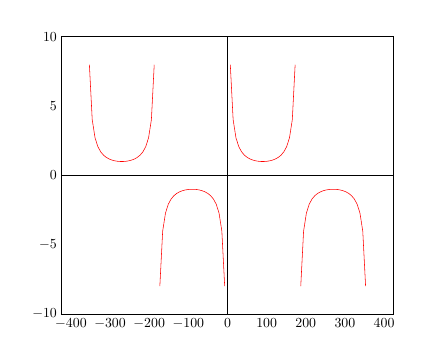
\begin{tikzpicture}[scale=0.5]
\begin{axis}[ymax=10,ymin=-10]
\addplot[color=red,domain=-360:360,samples=101,unbounded coords=jump]{cosec(x)};
\draw[ultra thin] (axis cs:0,\pgfkeysvalueof{/pgfplots/ymin}) -- (axis cs:0,\pgfkeysvalueof{/pgfplots/ymax});
\draw[ultra thin] (axis cs:\pgfkeysvalueof{/pgfplots/xmin},0) -- (axis cs:\pgfkeysvalueof{/pgfplots/xmax},0);
\end{axis}
\end{tikzpicture}
\\
$\cot(x)$
\\
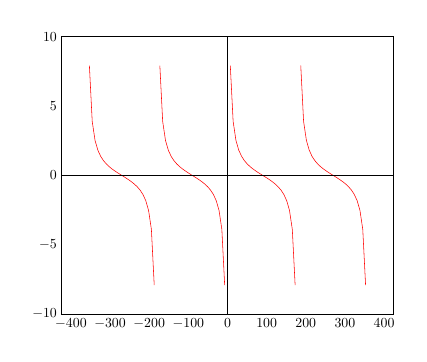
\begin{tikzpicture}[scale=0.5]
\begin{axis}[ymax=10,ymin=-10]
\addplot[color=red,domain=-360:360,samples=101,unbounded coords=jump]{cot(x)};
\draw[ultra thin] (axis cs:0,\pgfkeysvalueof{/pgfplots/ymin}) -- (axis cs:0,\pgfkeysvalueof{/pgfplots/ymax});
\draw[ultra thin] (axis cs:\pgfkeysvalueof{/pgfplots/xmin},0) -- (axis cs:\pgfkeysvalueof{/pgfplots/xmax},0);
\end{axis}
\end{tikzpicture}
\subsection{New identities}
\begin{itemize}
\item $1+\tan^2\theta=\sec^2\theta$
\item $1+\cot^2\theta=\csc^2\theta$
\end{itemize}
\subsection{Graphs of inverse functions}
$y=\arcsin(x)$
\\
\begin{tikzpicture}
  \begin{axis}[domain = -1:1, samples = 100,scale=0.5]
    \addplot[color = red]  {asin(x)/180*pi};
      \end{axis}
\end{tikzpicture}
\\
$y=\arccos(x)$
\\
\begin{tikzpicture}
  \begin{axis}[domain = -1:1, samples = 100,scale=0.5]
    \addplot[color = red]  {acos(x)/180*pi};
      \end{axis}
\end{tikzpicture}
\\
$y=\arctan(x)$
\\
\begin{tikzpicture}
  \begin{axis}[domain = -1:1, samples = 100,scale=0.5]
    \addplot[color = red]  {atan(x)/180*pi};
      \end{axis}
\end{tikzpicture}
\section{Further trigonometric identities and their applications}
\begin{itemize}
\item $\sin(a\pm b)\equiv\sin A\sin B\pm\cos A\sin B$
\item $\cos(a\pm b)\equiv\cos A\cos B\mp\sin A\sin B$
\item $\tan(a\pm b)\equiv\dfrac{\tan A\pm\tan B}{1\mp\tan A\tan B}$
\end{itemize}
\subsection{Double angle formulae}
\begin{itemize}
\item $\sin 2A\equiv 2\sin A\cos A$
\item $\cos 2A\equiv\cos^2A-\sin^2A\equiv 2\cos^2A-1\equiv 1-2\sin^2A$
\item $\tan 2A\equiv\dfrac{2\tan A}{1-\tan^2A}$
\end{itemize}
\subsection{The R formula}
For positive values of \textit{a} and \textit{b}
\\
$a\sin\theta\pm b\cos\theta$ can be expressed in the form $R\sin(\theta\pm\alpha)$, where $0<\alpha<90$
\\
$a\cos\theta\pm b\sin\theta$ can be expressed in the form $R\cos(\theta\mp\alpha)$, where $0<\alpha<90$ 
\\
$R\cos\alpha=a$, $R\sin\alpha=b$
\\
$R=\sqrt{a^2+b^2}$
\\
\section{Differentiation}
\subsection{The chain rule}
If $y=[f(x)]^n$ then $\dfrac{dy}{dx}=n[f(x)]^{n-1}f'x)$
\\
If $y=f[g(x)]$ then $\dfrac{dy}{dx}=f'[g(x)]g'(x)$
\\
\textbf{Example}
\\
$f(x)=(3x^4+x)^5$
\\
$f'(x)=12x^3+1$
\\
$\dfrac{dy}{dx}=5(3x^4+x)^4(12x^2+1)$
\\
\subsubsection{Another form of the chain rule}
$\dfrac{dy}{dx}=\dfrac{dy}{du}\times\dfrac{du}{dx}$
\\
\textbf{Example}
\\
$y=(x^2-7x)^4$
\\
$u=(x^2-7x)^4$
\\
$y=u^4$
\\
$\dfrac{du}{dx}=2x-7$\\
$\dfrac{dy}{du}=4u^3$\\
\textit{Using the chain rule:}\\
$\dfrac{dy}{dx}=4u^3\times(2x-7)$\\
$\dfrac{dy}{dx}=4(2x-7)(x^2-7x)^3$\\
\subsection{The product rule}
The product rule is used to differentiate the product of two functions.
\\
If $y=uv$ then $\dfrac{dy}{dx}=u\dfrac{dv}{dx}+v\dfrac{du}{dx}$
\\
\textbf{Example}:\\
$f(x)=x^2\sqrt{3x-1}$\\
$u=x^2$, $v=(3x-1)^{\frac{1}{2}}$\\
$\dfrac{du}{dx}=2x$ and $\dfrac{dv}{dx}=\dfrac{3}{2}(3x-1)^{-\frac{1}{2}}$\\
$f'(x)=x^2\times\frac{3}{2}(3x-1)^{-\frac{1}{2}}+\sqrt{3x-1}\times 2x$\\
$f'(x)=\dfrac{15x^2-4x}{2\sqrt{3x-1}}$\\
$f'(x)=\dfrac{x(15x-4)}{2\sqrt{3x-1}}$\\
\subsection{The quotient rule}
\
If $y=\dfrac{u(x)}{v(x)}$ then $\dfrac{dy}{dx}=\dfrac{v\dfrac{du}{dx}-u\dfrac{dv}{dx}}{v^2}$\\
\textbf{Example}\\
$y=\dfrac{x}{2x+5}$\\
$u=x, v=2x+5$\\
$\dfrac{du}{dx}=1$, $\dfrac{dv}{dx}=2$\\
$\dfrac{dy}{dx}=\dfrac{(2x+5)\times1-x\times2}{(2x+5)^2}$\\
$\dfrac{dy}{dx}=\dfrac{5}{(2x+5)^2}$\\
\subsection{The exponential function}
If $y=e^x$ then $\dfrac{dy}{dx}=e^x$\\
If $y=e^{f(x)}$ then $\dfrac{dy}{dx}=f'(x)e^{f(x)}$\\
\textbf{Example}\\
$y=e^{2x+3}$\\
$\dfrac{dy}{dx}2x+3=2$\\
$\dfrac{dy}{dx}e^{2x+3}=2e^{2x+3}$\\
\subsection{The logarithmic function}
If $y=\ln(x)$ then $\dfrac{dy}{dx}=\dfrac{1}{x}$\\
If $y=\ln[f(x)]$ then $\dfrac{dy}{dx}=\dfrac{f'(x)}{f(x)}$\\
\textbf{Example}\\
$y=\ln(6x-1)$\\
$\dfrac{dy}{dx}6x-1=6$\\
$\dfrac{dy}{dx}\ln(6x-1)=\dfrac{6}{6x-1}$
\subsection{Trig functions}
\subsubsection{Sin}
If $y=\sin(x)$ then $\dfrac{dy}{dx}=\cos(x)$\\
If $y=\sin f(x)$ then $\dfrac{dy}{dx}=f'(x)\cos f(x)$
\subsubsection{Cos}
If $y=\cos(x)$ then $\dfrac{dy}{dx}=-\sin(x)$\\
If $y=\cos f(x)$ then $\dfrac{dy}{dx}=-f'(x)\sin f(x)$\\
\subsubsection{Tan}
If $y=\tan(x)$ then $\dfrac{dy}{dx}=\sec^2(x)$\\
If $y=\tan f(x)$ then $\dfrac{dy}{dx}=f'(x)\sec^2f(x)$\\
\subsubsection{Csc}
If $y=\csc(x)$ then $\dfrac{dy}{dx}=-\csc(x)\cot(x)$\\
If $y=\csc f(x)$ then $\dfrac{dy}{dx}=-f'(x)\csc f(x)\cot f(x)$\\
\subsubsection{Sec}
If $y=\sec(x)$ then $\dfrac{dy}{dx}=\sec(x)\tan(x)$\\
If $y=\sec f(x)$ then $\dfrac{dy}{dx}=f'(x)\sec f(x)\tan f(x)$\\
\subsubsection{Cot}
If $y=\cot(x)$ then $\dfrac{dy}{dx}=-\csc^2(x)$\\
If $y=\cot f(x)$ then $\dfrac{dy}{dx}=-f'(x)\csc^2f(x)$\\
\newpage
\begin{center}
\underline{\huge Differentiation Table}
\end{center}



\begin{center}

\begin{Large}

\begin{tabular}{|c|c|}
 \hline
 $y$&$\dfrac{dy}{dx}$\\
 \hline
 $[f(x)]^n$&$n(f(x))^{n-1}f'(x)$\\
 \hline
 $uv$&$u\dfrac{dv}{dx}+v\dfrac{du}{dx}$\\
 \hline
 $\dfrac{f(x)}{g(x)}$&$\dfrac{f'(x)g(x)-f(x)g'(x)}{g(x)^2}$\\
 \hline
 $e^{f(x)}$&$f'(x)e^{f(x)}$\\
 \hline
 $\ln|f(x)|$&$\dfrac{f'(x)}{f(x)}$\\
 \hline
 $\sin f(x)$&$f'(x)\cos f(x)$\\
 \hline
 $\cos f(x)$&$-f'(x)\sin f(x)$\\
 \hline
 $\tan f(x)$&$f'(x)\sec^2f(x)$\\
 \hline
 $\csc f(x)$&$-f'(x)\csc f(x)\cot f(x)$\\
 \hline
 $\sec f(x)$&$f'(x)\sec f(x)\tan f(x)$\\
 \hline
 $\cot f(x)$&$-f'(x)\csc^2f(x)$\\
 \hline
\end{tabular}
\end{Large}
\end{center}




































\end{document}